\section{Installing Firefox on Windows}

\begin{enumerate}[1.]
\item
  To download Firefox, visit
  \href{https://www.mozilla.com/firefox/}{https://www.mozilla.com/firefox/}.
\end{enumerate}
\begin{figure}[htbp]
\centering
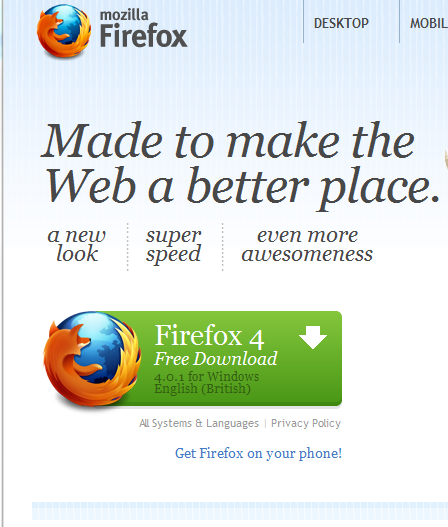
\includegraphics{ff_win_inst_1.png}
\caption{Windows Firefox Install}
\end{figure}

\begin{enumerate}[1.]
\setcounter{enumi}{1}
\item
  Click the download button and the installation file will begin to
  download to your computer.
\item
  Once the download is complete, double-click the installation file to
  start the Firefox installation wizard.

  \begin{itemize}
  \item
    If you are running Windows Vista, you may get a User Account Control
    prompt. In this case, allow the setup to run by clicking
    \textbf{Continue}.
  \item
    If you are running Windows 7, you will be asked whether to allow
    Firefox to make changes to your computer. Click on \textbf{Yes}.
  \end{itemize}
  A welcome screen appears.
\item
  Click \textbf{Next} to continue. You will be asked if you would like
  the standard installation, or whether you would like to customize it.
  Choose the standard installation and click \textbf{Next}.
\end{enumerate}
\begin{figure}[htbp]
\centering
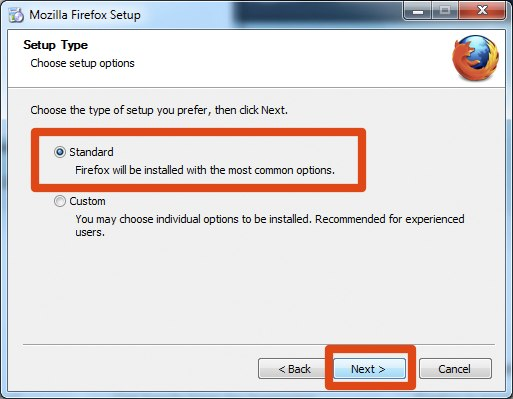
\includegraphics{ff_win_inst_2.png}
\caption{Windows Firefox Install}
\end{figure}

\begin{enumerate}[1.]
\setcounter{enumi}{4}
\item
  You will be asked if you want Firefox to be your default browser. This
  is recommended.
\end{enumerate}
\begin{figure}[htbp]
\centering
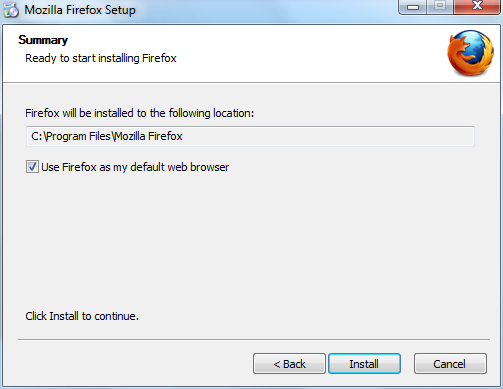
\includegraphics{ff_win_inst_3.png}
\caption{Windows Firefox Install}
\end{figure}

\begin{enumerate}[1.]
\setcounter{enumi}{5}
\item
  Click \textbf{Install}.
\item
  To import your bookmarks and other data from other browsers (for
  example Internet Explorer), click \textbf{Continue}. If you don't want
  to import anything, just select \textbf{Cancel}.
\end{enumerate}
\begin{figure}[htbp]
\centering
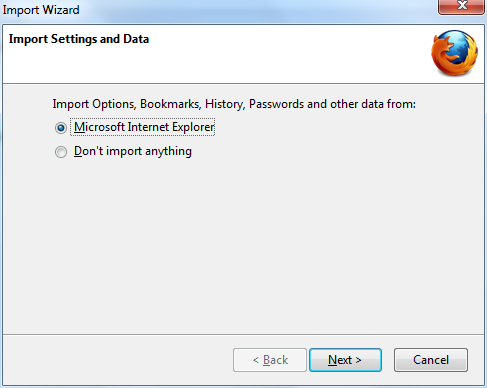
\includegraphics{ff_win_inst_4.png}
\caption{Windows Firefox Install}
\end{figure}

\begin{enumerate}[1.]
\setcounter{enumi}{7}
\item
  Once Firefox has been installed, click \textbf{Finish} to close the
  setup wizard.
\end{enumerate}
If the \textbf{Launch Firefox now} check box is checked, Firefox will
start after you click \textbf{Finish}. Otherwise you can launch Firefox
through the start menu.

\subsubsection{Windows Vista Users}

If at any time throughout the installation process you are prompted with
a User Account Control (UAC) window, press Continue, Allow, or Accept.

\subsection{Troubleshooting}

If you have problems starting Firefox, see
\href{https://support.mozilla.com/kb/Firefox+will+not+start}{https://support.mozilla.com/kb/Firefox+will+not+start}
